\documentclass[12p]{report}
\usepackage[T1]{fontenc}
\usepackage[utf8]{inputenc}
\usepackage{graphicx} 
\usepackage{float}
\linespread{1.5}
\begin{document}

\tableofcontents
\newpage
\quad Celem pracy jest przedstawienie algorytmów kryptograficznych oraz możliwych ataków. Następnie implementacja 2 algorytmów na systemie wbudowanym oraz porównanie ich wydajności w zależności od rozmiaru szyfrowanych danych.
\newpage


%-----------------------------------
%	Rozdział 1
%-----------------------------------
\chapter{Kryptologia}
\section{Wprowadzenie}

\quad W obecnych czasach dużym zainteresowaniem cieszy się bezpieczeństwo cybernetyczne, którego szczególną częścią jest kryptografia. Szczególnie ważne zastosowanie znajduje w branży informatycznych, militarnej, urzędach, grupach developerskich czy bankowości. Kryptografia pojawiła się znaczniej wcześniej niż platformy obliczeniowe, zainteresowali się nią już ludzie z czasów starożytnych, pojawiła się wraz z umiejętnością pisania. Powodem istnienia kryptografii jest bezpieczne i prywatne dostarczanie wiadomości. Znajduje szczególne zastosowanie w przypadku danych przesyłanych drogą komunikacyjną. W obecnych czasach powszechną drogą komunikacyjną jest droga internetowa, dzięki kryptografii możliwe jest zapewnienie bezpieczeństwa cybernetycznego przesyłanych danych. W zależności od stopnia poufności informacji, którą chcemy zaszyfrować, aby niepożądane osoby jej nie odczytały można zastosować odmiennych algorytmów szyfrowania. 

\quad Kryptologia to połączenie kryptografii i kryptoanalizy. W języku greckim 'kryptos' oznacza ukryty, zaś 'logos' tłumaczone jest jako słowo. Kryptologia jest dziedziną zajmującą się ukrywaniem tekstu jawnego. Kryptografia jest dziedziną węższą od kryptologii, jest badaniem technik matematycznych związanych z bezpieczeństwem informacji. Do bezpieczeństwa danych można zaliczyć poufność informacji, uwierzytelnienie użytkowników i pochodzenia danych, a także integralność danych. Słowo kryptologia składa się z dwóch greckich słów: 'kryptos' znaczący ukryty i 'graph' oznaczający pisanie, jest to nauka o zabezpieczaniu danych. Za pomocą technik kryptograficznych możliwe jest zaszyfrowanie jawnego tekstu, w taki sposób aby niepożądana osoba nie mogła ich odczytać. Drugą gałęzią kryptologii jest kryptoanaliza, która zajmuje się analizą i możliwymi sposobami odszyfrowania kodu kryptograficznego.
\subsection{Terminologia kryptologiczna}
frfefe

\section{Maszyna Enigma}

\section{Szyfry blokowe i strumieniowe}
\subsection{Szyfry blokowe} 
\quad Szyfry blokowe wykorzystywane są do szyfrowania i deszyfrowania. Danymi wejściowymi do szyfrowania jest blok danych, który przy użyciu klucza szyfrującego jest przekształcany w zaszyfrowany blok danych. Odszyfrowywanie przebiega w odwrotny sposób, zaszyfrowana blokowa wiadomość przy użyciu klucza jest transformowana do odszyfrowanej blokowej wiadomości. Szyfr blokowy jest bezpieczny do momentu kiedy klucz szyfrujący pozostaje tajny. Bez znajomości klucza niemożliwe staje się rozszyfrowanie wiadomości w satysfakcjonującym nas czasie. Im bardziej klucz jest przypadkowy tym ciężej złamać algorytm. Ważnymi parametrami szyfru blokowego jest rozmiar bloku i klucza od których to zależy bezpieczeństwo algorytmu. Powszechnie stosowanymi rozmiarami bloków są 64 i 128 bitowe bloki, zazwyczaj algorytm DES ma 64 bitowy blok danych, zaś AES 128 bitowy blok. 
\begin{figure}[h]
\centering
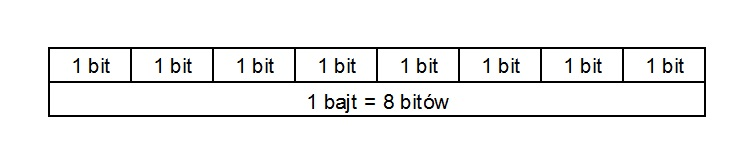
\includegraphics[width=12cm]{bajt.jpg}
\caption{Tu umieszczasz opis}
\end{figure}

\quad Długość zaszyfrowanego bloku musi być optymalna, im większe bloki danych tym dłuższy zaszyfrowany tekst oraz użycie pamięci. Przy szyfrowaniu wiadomości która na długość 8 bitową, zaś blok szyfru ma długość 64 bity najpierw 8 bitowa wiadomość zostanie prze konwertowana na 64 bitowy blok. Następnie 64 bitowa wiadomość zostanie zaszyfrowana przy użyciu algorytmu tworząc zaszyfrowany tekst. Do przetworzenia szyfru blokowego o rozmiarze 64 bitów potrzebujemy 64 bitów pamięci w rejestrach procesora. W dzisiejszych czasach procesory z pamięcią 64 bitową nie są kosztowne, lecz im większy chcemy utworzyć blok szyfrowy tym lepszy procesor potrzebujemy, co może mieć znaczny wpływ na wysokie koszty.
\subsubsection{Powszechne ataki}

\section{Szyfry symetryczne i asymetryczne}
\subsection{Szyfry symetryczne}
\subsubsection{DES}
\subsubsection{AES}
\subsubsection{IDEA}
\subsubsection{Blowfish}
\subsection{Szyfry asymetryczne}
\subsubsection{RSA}
\subsubsection{DSS(DSA)}
\subsubsection{Diffie-Hellman}



\end{document}
